\section{Trabajo Extra: Refinamiento de Historias Grandes}

\subsection{Criterios y Justificación de la Descomposición Ágil}

En el desarrollo de software ágil, una historia de usuario valorada en 13 o 21 Story Points constituye un \textbf{antipatrón} para la planificación de sprints por múltiples razones:
\begin{enumerate}
    \item \textbf{Violación del principio INVEST (\textit{Small}):} Una historia de 13 o 21 puntos excede con creces la capacidad de absorción y el margen de seguridad de una iteración estándar de dos semanas en un equipo universitario.
    \item \textbf{Efecto binario \enquote{Todo o Nada}:} Si un requerimiento masivo se traba en su fase final de pruebas o despliegue, la historia completa pasa al siguiente sprint con 0 puntos entregados, arruinando la predictibilidad de la velocidad del equipo.
    \item \textbf{Incertidumbre enmascarada:} Los puntajes elevados suelen ser un síntoma de que el requerimiento es en realidad una \textbf{Épica camuflada} que engloba flujos alternativos, reglas de negocio no analizadas y riesgos de integración no dimensionados.
\end{enumerate}

Para corregir esta situación, el equipo sometió las cuatro historias complejas (\texttt{HU-03}, \texttt{HU-05}, \texttt{HU-07} y \texttt{HU-11}) a un proceso formal de refinamiento (*Backlog Refinement*), aplicando patrones de división reconocidos en la industria (marco SPIDR y división por reglas de negocio/flujos):

\begin{itemize}
    \item \textbf{División por rol y secuencia del flujo (\texttt{HU-03}):} La marcación de asistencia QR involucra dos actores con necesidades asimétricas. Se descompuso en lo que compete al docente (generación del código QR dinámico proyectado), lo que compete al participante (escaneo y validación desde la cámara web/móvil) y la capa de control antifraude (bloqueo de duplicados y visualización de la nómina de presentes en tiempo real).
    \item \textbf{División por reglas de negocio y valor incremental (\texttt{HU-05}):} La emisión de certificados se fragmentó desacoplando la lógica de validación previa (cálculo de notas y umbral de asistencia), la renderización física del PDF vectorial con firma y hash SHA-256 para un alumno individual, y el subsistema de procesamiento por lotes (*batch job*) para emitir masivamente todos los diplomas de un curso al término del acta.
    \item \textbf{División por capas de valor y alcance operativo (\texttt{HU-07}):} En la gestión multientidad se independizó la creación básica de la entidad institucional (datos fiscales y logo), la asociación relacional de usuarios y capacitaciones a dicha entidad, y la implementación rigurosa de los filtros globales de aislamiento de datos en las consultas Eloquent.
    \item \textbf{Técnica del Spike Técnico con tiempo delimitado (\texttt{HU-11}):} Dado que el modo offline representaba una barrera tecnológica desconocida para el equipo, se aisló en primera instancia un \textbf{Spike de Investigación (2 SP)}. Este spike no busca entregar código productivo, sino un prototipo descartable para evaluar la viabilidad de la API de \textit{Service Workers} e \textit{IndexedDB}. Una vez desarmada la incertidumbre, el almacenamiento local, la sincronización en segundo plano y los indicadores visuales pudieron dimensionarse con total confianza.
\end{itemize}

Cada historia hija resultante fue formulada manteniendo la sintaxis estándar \textit{Como / Quiero / Para}, provista de criterios de aceptación propios y re-estimada en equipo bajo la misma baraja de Fibonacci.

\subsection{Historias Refinadas y Re-estimación en Jira}

La Tabla~\ref{tab:historias_refinadas} detalla la correspondencia entre las cuatro historias padre originales, sus historias hijas creadas en Jira Software (claves \texttt{SC-28} a \texttt{SC-40}), los nuevos puntajes de Story Points asignados y su clasificación.

\begin{table}[H]
\centering
\small
\renewcommand{\arraystretch}{1.18}
\caption{Matriz de refinamiento y re-estimación de las historias complejas (etiquetadas como \texttt{refinamiento} en Jira).}
\label{tab:historias_refinadas}
\begin{tabularx}{\textwidth}{P{1.2cm} P{2.0cm} P{1.2cm} P{1.4cm} Y C{1.2cm} C{2.2cm}}
\toprule
\rowcolor{headerblue}
\textcolor{white}{\textbf{Clave}} & \textcolor{white}{\textbf{Origen (SP)}} & \textcolor{white}{\textbf{Nueva}} & \textcolor{white}{\textbf{Código}} & \textcolor{white}{\textbf{Historia de Usuario Refinada}} & \textcolor{white}{\textbf{SP}} & \textcolor{white}{\textbf{Tipo}} \\
\midrule
\rowcolor{white}
\textbf{SC-14} & \textbf{HU-07} & SC-28 & HU-07.1 & Registrar institución con RUC, razón social y logo & 3 & \badgeCorta \\
\rowcolor{white}
& \textit{(13 SP)} & SC-29 & HU-07.2 & Asociar usuarios y capacitaciones a una institución & 5 & \badgeMedia \\
\rowcolor{white}
& & SC-30 & HU-07.3 & Aislar los datos para que cada institución vea lo suyo & 5 & \badgeMedia \\
\rowcolor{rowalt}
\multicolumn{5}{r}{\textbf{Subtotal refinado HU-07:}} & \textbf{13 SP} & \textit{3 historias} \\
\midrule
\rowcolor{white}
\textbf{SC-20} & \textbf{HU-03} & SC-31 & HU-03.1 & Generar QR dinámico por sesión (vista docente) & 5 & \badgeMedia \\
\rowcolor{white}
& \textit{(13 SP)} & SC-32 & HU-03.2 & Registrar asistencia escaneando el QR (participante) & 5 & \badgeMedia \\
\rowcolor{white}
& & SC-33 & HU-03.3 & Evitar marcaciones duplicadas y ver lista de sesión & 3 & \badgeCorta \\
\rowcolor{rowalt}
\multicolumn{5}{r}{\textbf{Subtotal refinado HU-03:}} & \textbf{13 SP} & \textit{3 historias} \\
\midrule
\rowcolor{white}
\textbf{SC-22} & \textbf{HU-05} & SC-34 & HU-05.1 & Validar requisitos de emisión (nota $\ge 11$ y asistencia) & 3 & \badgeCorta \\
\rowcolor{white}
& \textit{(13 SP)} & SC-35 & HU-05.2 & Generar PDF con plantilla, QR vectorial y hash SHA-256 & 5 & \badgeMedia \\
\rowcolor{white}
& & SC-36 & HU-05.3 & Emitir certificados en lote para todo un curso & 5 & \badgeMedia \\
\rowcolor{rowalt}
\multicolumn{5}{r}{\textbf{Subtotal refinado HU-05:}} & \textbf{13 SP} & \textit{3 historias} \\
\midrule
\rowcolor{white}
\textbf{SC-27} & \textbf{HU-11} & SC-37 & HU-11.1 & Spike: evaluar almacenamiento local (PWA + IndexedDB) & 2 & \badgeCorta \\
\rowcolor{white}
& \textit{(21 SP)} & SC-38 & HU-11.2 & Guardar asistencias en el dispositivo en modo offline & 5 & \badgeMedia \\
\rowcolor{white}
& & SC-39 & HU-11.3 & Sincronizar asistencias pendientes al reconectar sin duplicados & 8 & \badgeMedia \\
\rowcolor{white}
& & SC-40 & HU-11.4 & Mostrar indicador visual de datos pendientes de sincronizar & 3 & \badgeCorta \\
\rowcolor{rowalt}
\multicolumn{5}{r}{\textbf{Subtotal refinado HU-11:}} & \textbf{18 SP} & \textit{4 historias} \\
\midrule
\rowcolor{headerblue!10}
\multicolumn{5}{r}{\textbf{Total Refinado (13 historias hijas):}} & \textbf{57 SP} & \textit{Reducción de riesgo} \\
\bottomrule
\end{tabularx}
\end{table}

La Figura~\ref{fig:refinamiento_historias} sintetiza visualmente este desglose estructural, mostrando cómo cada historia original compleja fue desmembrada y re-estimada en Jira.

\begin{figure}[H]
    \centering
    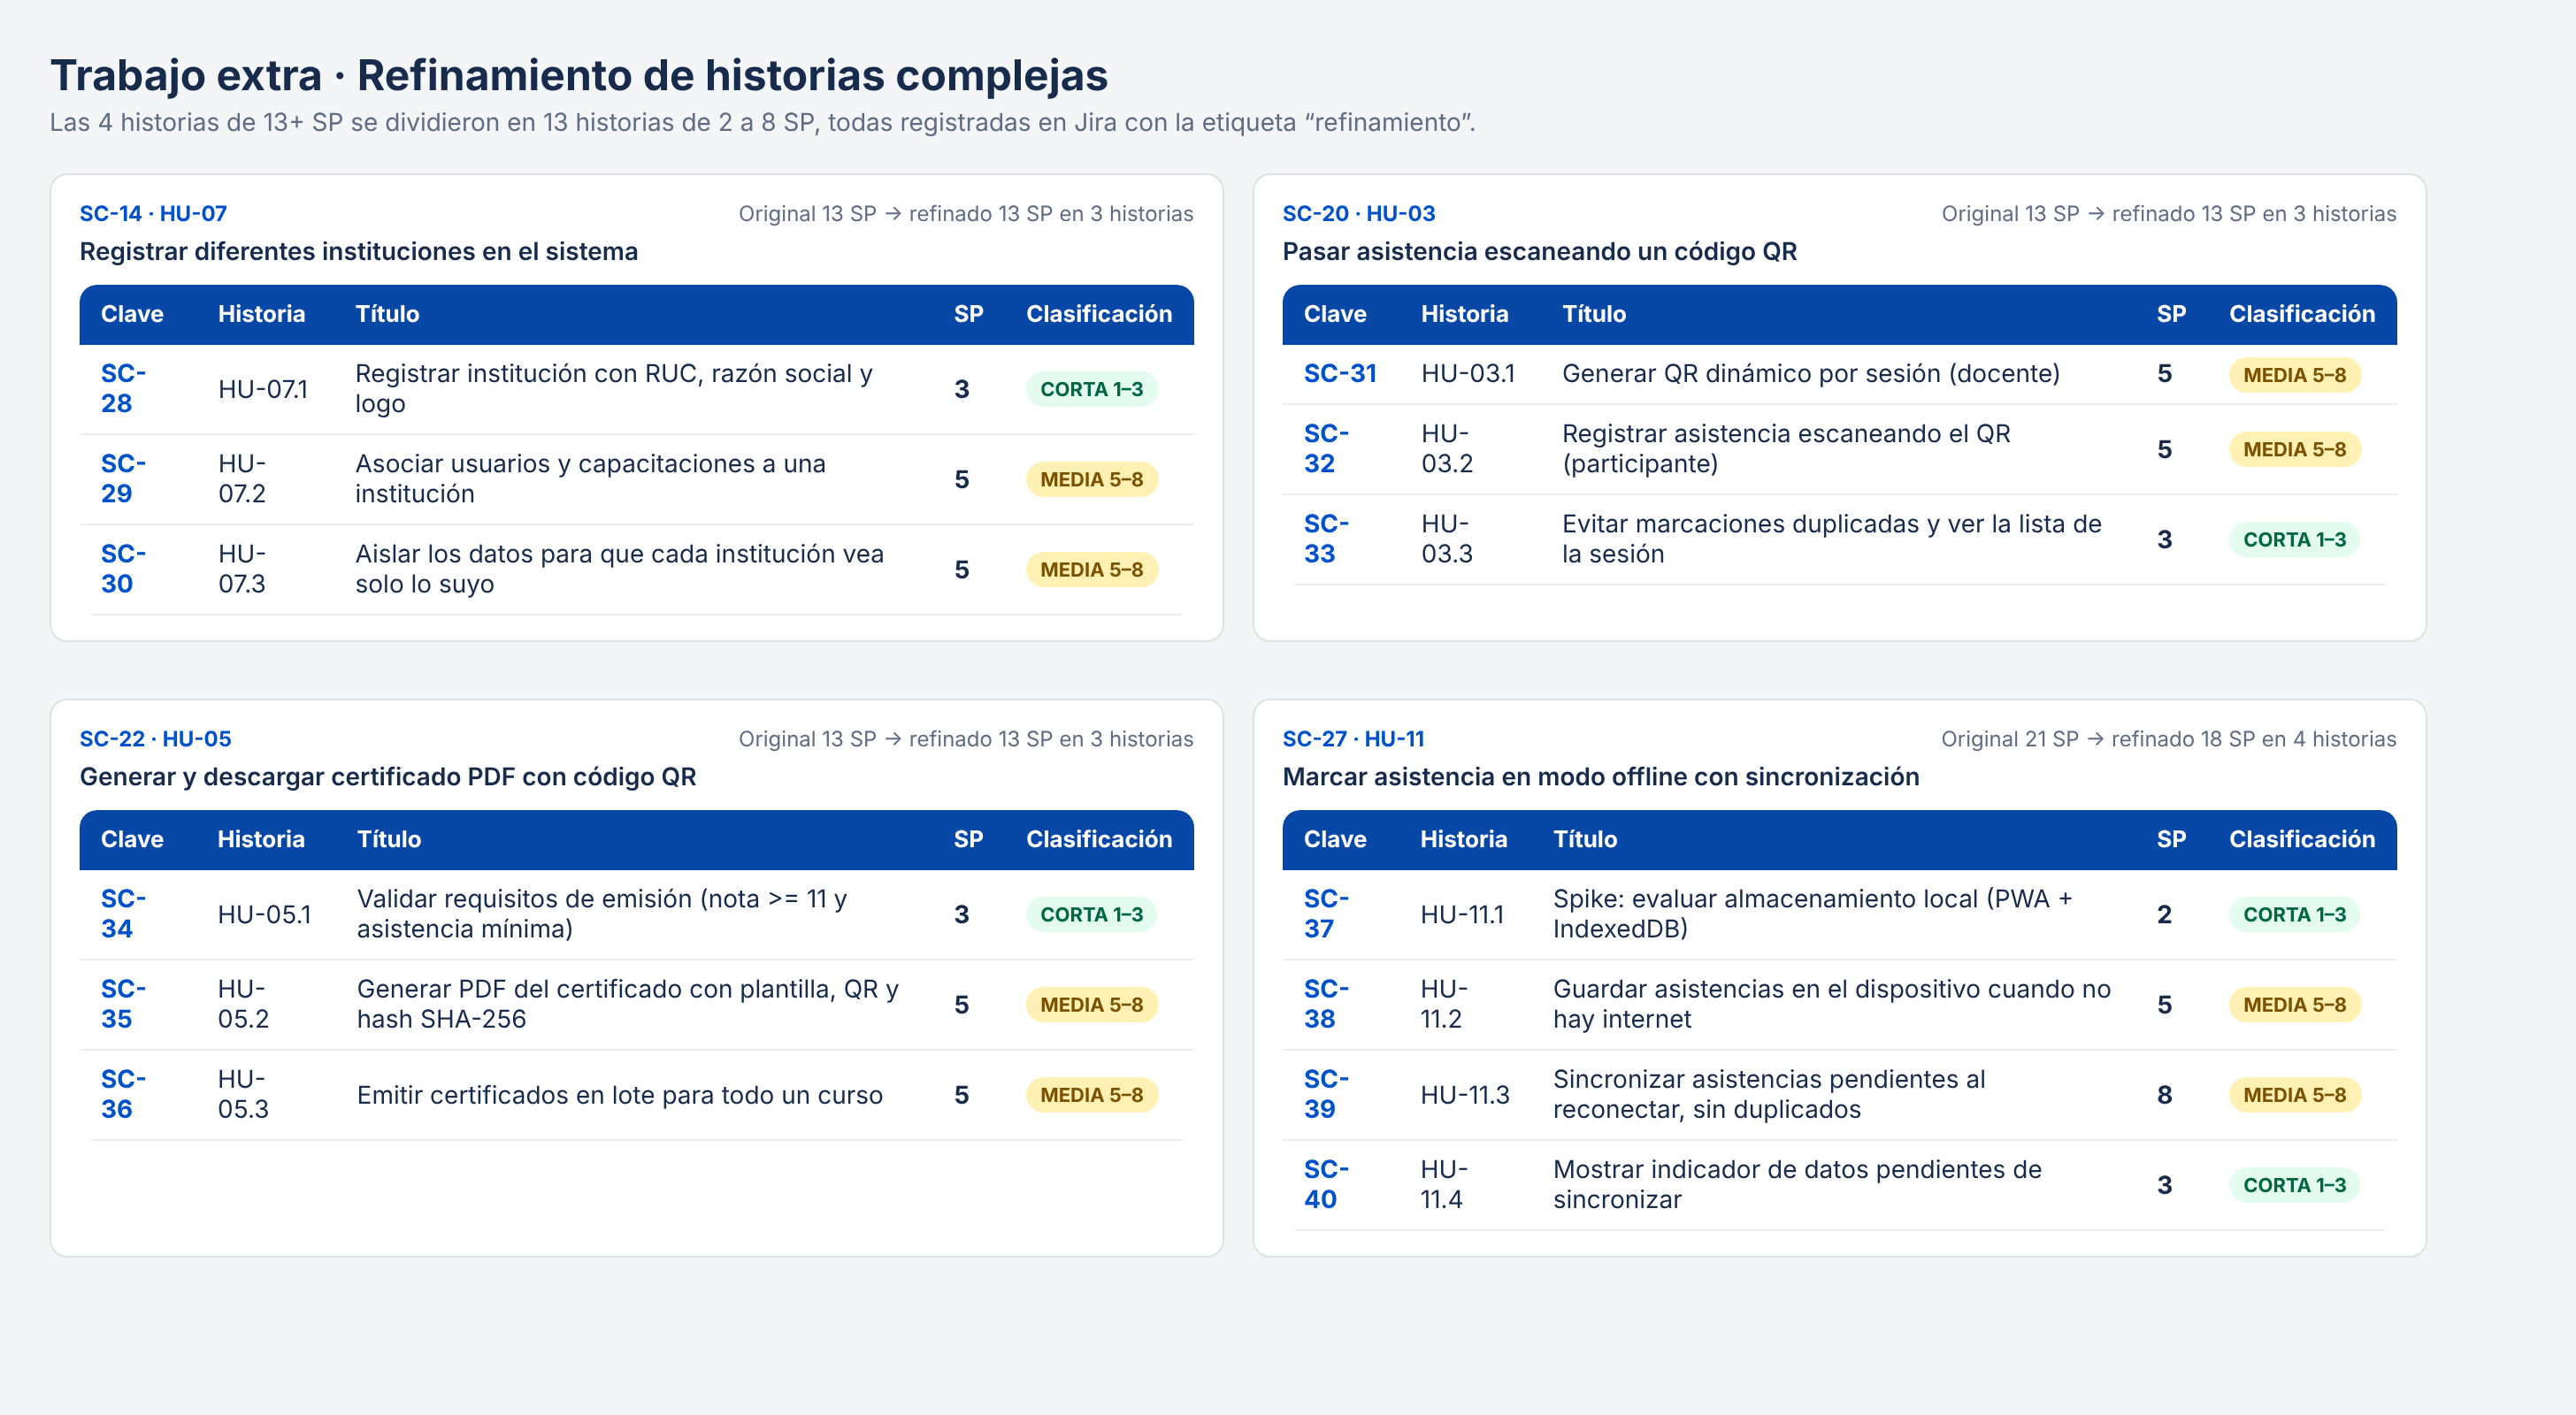
\includegraphics[width=\textwidth]{figura6_refinamiento_historias.png}
    \caption{Evidencia gráfica del trabajo extra: descomposición de las cuatro historias complejas de 13+ SP en 13 historias atómicas de 2 a 8 SP, con sus respectivas claves Jira y puntajes.}
    \label{fig:refinamiento_historias}
\end{figure}

\subsection{Impacto Cuantitativo y Cualitativo del Refinamiento}

El ejercicio de refinamiento generó un impacto positivo inmediato en la salud del Product Backlog:

\begin{enumerate}
    \item \textbf{Eliminación absoluta de historias no planificables:} Las 4 historias complejas (que sumaban 60 SP de alto riesgo) se convirtieron en 13 historias manejables que oscilan entre 2 y 8 SP. \textbf{En el backlog activo del SIGC-CUSCO ya no existe ninguna historia que supere los 8 Story Points}. Todas caben holgadamente dentro de una iteración y pueden ser probadas de manera autónoma.
    
    \item \textbf{Ahorro y precisión mediante el Spike Técnico (\texttt{HU-11}):} El requerimiento de sincronización offline redujo su estimación total de \textbf{21 a 18 SP}. Al separar formalmente el spike técnico (\texttt{HU-11.1} con 2 SP), el equipo aisló la fase de experimentación y prueba de concepto; las tres historias de implementación subsiguientes se estimaron sobre certezas funcionales (guardado local con 5 SP, sincronización con 8 SP y semáforo visual con 3 SP), eliminando el colchón de incertidumbre que inflaba la historia original.
    
    \item \textbf{Composición final del Backlog Activo:} Al sustituir las 4 historias padre por sus 13 hijas, el backlog operativo queda constituido por \textbf{22 historias de usuario} (9 historias originales no complejas + 13 historias refinadas). El esfuerzo global activo se ajustó de 99 a \textbf{96 Story Points}:
    \begin{itemize}
        \item \textbf{Historias Cortas (1--3 SP):} 10 historias (26 SP, 27.1\% del backlog).
        \item \textbf{Historias Medias (5--8 SP):} 12 historias (70 SP, 72.9\% del backlog).
        \item \textbf{Historias Complejas (13+ SP):} \textbf{0 historias activas} (0\%).
    \end{itemize}
    
    \item \textbf{Política de trazabilidad en Jira:} Las cuatro historias padre originales (\texttt{SC-14}, \texttt{SC-20}, \texttt{SC-22} y \texttt{SC-27}) se conservaron en Jira con el estado de cerradas por división, etiquetadas como \texttt{dividida} y vinculadas con enlaces de issue (\textit{\enquote{is parent of}}) hacia sus respectivas hijas. Esto preserva el historial de la estimación original como evidencia académica y de auditoría de procesos.
\end{enumerate}
